\documentclass{article}

\usepackage{amsmath, amsthm, amssymb, amsfonts}
\usepackage{thmtools}

% ------------------------------------------------------------------------------
\usepackage{graphicx}
\graphicspath{ {./images/} }
% ------------------------------------------------------------------------------

\usepackage{setspace}
\usepackage{geometry}
\usepackage{float}
\usepackage{hyperref}
\usepackage[english]{babel}
\usepackage{framed}
\usepackage[dvipsnames]{xcolor}
\usepackage{tcolorbox}
\usepackage{minted}

% ------------------------------------------------------------------------------
% \usepackage{times}
% \usepackage{fontspec}
% \setmainfont{Ubuntu Nerd Font}
% \setsansfont{Noto Sans}
% \setmonofont{FiraCode Nerd Font}
% ------------------------------------------------------------------------------

\colorlet{LightGray}{White!90!Periwinkle}
\colorlet{LightOrange}{Orange!15}
\colorlet{LightGreen}{Green!15}

\newcommand{\HRule}[1]{\rule{\linewidth}{#1}}

\declaretheoremstyle[name=Theorem,]{thmsty}
\declaretheorem[style=thmsty,numberwithin=section]{theorem}
\tcolorboxenvironment{theorem}{colback=LightGray}

\declaretheoremstyle[name=Proposition,]{prosty}
\declaretheorem[style=prosty,numberlike=theorem]{proposition}
\tcolorboxenvironment{proposition}{colback=LightOrange}

\declaretheoremstyle[name=Principle,]{prcpsty}
\declaretheorem[style=prcpsty,numberlike=theorem]{principle}
\tcolorboxenvironment{principle}{colback=LightGreen}

\setstretch{1.2}
\geometry{
    textheight=9in,
    textwidth=5.5in,
    top=1in,
    headheight=12pt,
    headsep=25pt,
    footskip=30pt
}

% ------------------------------------------------------------------------------

\begin{document}

% ------------------------------------------------------------------------------
% Cover Page and ToC
% ------------------------------------------------------------------------------

\title{ \normalsize \textsc{}
\\ [2.0cm]
\HRule{1.5pt} \\
\LARGE \textbf{\uppercase{Data Communications and
	Networking}
\HRule{2.0pt} \\ [0.6cm] \LARGE{Chapter 08} \vspace*{10\baselineskip}}
}
\date{}
\author{\textbf{Rising Flare Community} \\
	Made with ArchLinux and vscode (\LaTeX workshop).
}

\maketitle
\begin{center}
	Source code is available on \href{https://github.com/SharafatKarim/pstu-cse-academic/blob/main/semester%203/cce/networking%20exercises/ch%208/cce_ch8.tex}{GitHub}. 
	Feel free to do changes or improvements. Use xetex to compile the tex file instead of using \LaTeX directly for avoiding font issues.
\end{center}
\newpage

\tableofcontents
\newpage

% ------------------------------------------------------------------------------

\section{Questions}
\subsection{
	Describe the need for switching and define a switch.
}
A switched network consists of a series of interlinked nodes, called switches.
Switching is required to connect multiple devices to a single network. \\
A switch is a device that connects multiple devices to a single network. For example, routers, bridges, and gateways are all types of switches.
\subsection{
	List the three traditional switching methods. Which are the most common
	today?
}
The three traditional switching methods are
\begin{itemize}
	\item Circuit switching
	\item Message switching
	\item Packet switching
\end{itemize}
Circuit switching and Packet switching is the most common method today.
\subsection{
	What are the two approaches to packet switching?
}
The two approaches to packet switching are datagram and virtual-circuit.
\subsection{
	Compare and contrast a circuit-switched network and a packet-switched network.
}
In a circuit-switched network, a dedicated communication path is established between two devices. 
In a packet-switched network, data is divided into packets and sent over the network.
\subsection{
	What is the role of the address field in a packet traveling through a datagram
	network?
}
The address field in a packet traveling through a datagram network is used to identify the destination device.
\subsection{
	What is the role of the address field in a packet traveling through a virtual-
	circuit network?
}
The address field in a packet traveling through a virtual-circuit network is used to identify the virtual circuit.
\subsection{
	Compare space-division and time-division switches.
}
Space-division switches use multiple paths to connect devices, while time-division switches use a single path and divide the time into slots.
\subsection{
	What is TSI and what is its role in time-division switching?
}
TSI stands for Time Slot Interchange. It is used to switch time slots in a time-division switch.
\subsection{
	Compare and contrast the two major categories of circuit switches.
}
The two major categories of circuit switches are crossbar switches and time-division switches. 
Crossbar switches use multiple paths to connect devices, while time-division switches use a single path and divide the time into slots.
\subsection{
	List four major components of a packet switch and their functions.
}
The four major components of a packet switch are
\begin{itemize}
	\item Input ports
	\item Output ports
	\item Switching fabric
	\item Routing processor
\end{itemize}

% ------------------------------------------------------------------------------
% ------------------------------------------------------------------------------
% ------------------------------------------------------------------------------
\section{Problems}
\subsection{
	A path in a digital circuit-switched network has a data rate of 1 Mbps. The exchange of 1000 bits is required for the setup and teardown phases. 
	The distance between two parties is 5000 km. Answer the following questions if the propagation speed is
	\texorpdfstring{$ 2 \times 10^8 $}{2 x 10^8} m.
}

\textbf{
	\begin{enumerate}
		\item What is the total delay if 1000 bits of data are exchanged during the data-transfer phase?
		\item What is the total delay if 100,000 bits of data are exchanged during the data-transfer phase?
		\item What is the total delay if 1,000,000 bits of data are exchanged during the data-transfer phase?
		\item Find the delay per 1000 bits of data for each of the above cases and compare them. What can you infer?
	\end{enumerate}
}

Here, in the setup phase we have to exchange data two times, and once for the teardown. \par
Propagation delay = $ \frac{ 5000 \times 10^3 }{ 2 \times 10 ^8 } = 0.025 sec $ \par
Transmission delay = $ \frac{ 1000 }{ 10^6 } = 0.001 sec $ \\
So, delay for setup and teardown phase = $ 0.025 \times 3 + 0.001 \times 3 = 0.078 sec $  \par

\begin{enumerate}
	\item For 1000 bits of data, total delay = $ 0.078 + 0.025 + \frac{ 1000 }{ 10^6 } = 0.104 sec $
	\item For 100,000 bits of data, total delay = $ 0.078 + 0.025 + \frac{ 100000 }{ 10^6 } = 0.203 sec $
	\item For 1,000,000 bits of data, total delay = $ 0.078 + 0.025 + \frac{ 1000000 }{ 10^6 } = 1.103 sec $
	\item For above cases,
	      \begin{enumerate}
		      \item For 1000 bits delay will be, $ \frac{0.104 \times 1000}{1000} = 0.104 sec $
		      \item For 1000 bits delay will be, $ \frac{0.203 \times 1000}{100000} = 0.00203 sec $
		      \item For 1000 bits delay will be, $ \frac{1.103 \times 1000}{1000000} = 0.001103 sec $
	      \end{enumerate}
	      The ratio for case c is the smallest because we use
	      one setup and teardown phase to send more data.
\end{enumerate}


\subsection{Five equal-size datagrams belonging to the same message leave for the destination one after another. However, they travel through different paths as
	shown in Table 1.
}
\begin{table}[H]
	\centering
	\begin{tabular}{ | c | c | c | }
		\hline
		Datagram & Path Length & Visited Switches \\
		\hline
		1        & 3200 km     & 1, 3, 5          \\
		\hline
		2        & 11,700 km   & 1, 2, 5          \\
		\hline
		3        & 12,200 km   & 1, 2, 3, 5       \\
		\hline
		4        & 10,200 km   & 1, 4, 5          \\
		\hline
		5        & 10,700 km   & 1, 4, 3, 5       \\
		\hline
	\end{tabular}
	\caption{P8-2}
	\label{table:1}
\end{table}
\textbf{
	We assume that the delay for each switch (including waiting and processing)
	is 3, 10, 20, 7, and 20 ms respectively. Assuming that the propagation speed is
	$2 \times 10^8$ m, find the order the datagrams arrive at the destination and the delay
	for each. Ignore any other delays in transmission.
}

Here, let's assume all datagrams start at the same time. \\
Arrival time for datagram 1 = $ \frac{3200 \times 10^3}{2 \times 10^8} + (3 + 20 + 20) = 0.059 sec $ \\
Arrival time for datagram 2 = $ \frac{11700 \times 10^3}{2 \times 10^8} + (3 + 10 + 20) = 0.0915 sec $ \\
Arrival time for datagram 3 = $ \frac{12200 \times 10^3}{2 \times 10^8} + (3 + 10 + 20 + 20) = 0.114 sec $ \\
Arrival time for datagram 4 = $ \frac{10200 \times 10^3}{2 \times 10^8} + (3 + 7 + 20) = 0.081 sec $ \\
Arrival time for datagram 5 = $ \frac{10700 \times 10^3}{2 \times 10^8} + (3 + 7 + 20 + 20) = 0.1035 sec $ \par
The order of arrival is 1, 4, 2, 5, 3. First datagram 1 arrives, then datagram 4, then datagram 2, then datagram 5, and finally datagram 3. \par

\subsection{
	Transmission of information in any network involves end-to-end addressing
	and sometimes local addressing (such as VCI). Table 8.2 shows the types of
	networks and the addressing mechanism used in each of them.
}
\begin{table}[H]
	\centering
	\begin{tabular}{ | c | c | c | c | }
		\hline
		Network          & Setup      & Data Transfer & Teardown   \\
		\hline
		Circuit-switched & End-to-end &               & End-to-end \\
		\hline
		Datagram         &            & End-to-end    &            \\
		\hline
		Virtual-Circuit  & End-to-end & Local         & End-to-end \\
		\hline
	\end{tabular}
	\caption{P8-3}
	\label{table:2}
\end{table}

\textbf{
	Answer the following questions:
}
\begin{enumerate}
	\item \textbf{ Why does a circuit-switched network need end-to-end addressing during the
		      setup and teardown phases? Why are no addresses needed during the data
		      transfer phase for this type of network? } \\
	      It's because in a circuit-switched network, a dedicated communication path is established between two devices. The addresses are needed during the setup and teardown phases to establish and release the connection. No addresses are needed during the data transfer phase because the connection is already established.

	\item \textbf{Why does a datagram network need only end-to-end addressing during the
		      data transfer phase, but no addressing during the setup and teardown phases? } \\
	      In a datagram network, data is divided into packets and sent over the network. The addresses are needed during the data transfer phase to identify the destination device. No addresses are needed during the setup and teardown phases because the packets are sent independently.

	\item \textbf{  Why does a virtual-circuit network need addresses during all three phases? }
	      In a virtual-circuit network, a connection is established between two devices using a virtual circuit. The addresses are needed during all three phases to establish, transfer data, and release the connection. And also, the local addressing is needed to identify the virtual circuit.
\end{enumerate}

\subsection{We mentioned that two types of networks, datagram and virtual-circuit, need a
	routing or switching table to find the output port from which the information
	belonging to a destination should be sent out, but a circuit-switched network
	has no need for such a table. Give the reason for this difference. }

In a circuit-switched network, a dedicated communication path is established between two devices. The path is already established, so there is no need for a routing or switching table. In datagram and virtual-circuit networks, the information is sent over the network and the output port needs to be found using a routing or switching table.

\subsection{An entry in the switching table of a virtual-circuit network is normally created
	during the setup phase and deleted during the teardown phase. In other words,
	the entries in this type of network reflect the current connections, the activity
	in the network. In contrast, the entries in a routing table of a datagram network
	do not depend on the current connections; they show the configuration of the
	network and how any packet should be routed to a final destination. The
	entries may remain the same even if there is no activity in the network. The
	routing tables, however, are updated if there are changes in the network. Can
	you explain the reason for these two different characteristics?
	Can we say that a virtual-circuit is a connection-oriented network and a datagram network is a
	connectionless network because of the above characteristics?}

In a virtual-circuit network, a connection is established between two devices using a virtual circuit.
The entries in the switching table reflect the current connections in the network. In a datagram network, data is divided into packets and sent over the network.
The entries in the routing table show the configuration of the network and how any packet should be routed to a final destination.
The entries may remain the same even if there is no activity in the network.
The routing tables are updated if there are changes in the network.
A virtual-circuit network is a connection-oriented network because a connection is established between two devices using a virtual circuit.
A datagram network is a connectionless network because data is divided into packets and sent over the network.

\begin{proposition}
	In circuit-switched and virtual-circuit networks, we are dealing with connections.
	A connection needs to be made before the data transfer can take place. In the case
	of a circuit-switched network, a physical connection is established during the setup
	phase and the is broken during the teardown phase. \\ In the case of a virtual-circuit
	network, a virtual connection is made during setup and is broken during the tear-
	down phase; the connection is virtual, because it is an entry in the table. These two
	types of networks are considered connection-oriented. In the case of a datagram
	network no connection is made. Any time a switch in this type of network receives
	a packet, it consults its table for routing information. This type of network is con-
	sidered a connectionless network.
\end{proposition}

\begin{theorem}
	A virtual-circuit is a connection-oriented network and a datagram network is a
	connectionless network.
\end{theorem}

\subsection{The minimum number of columns in a datagram network is two; the minimum
	number of columns in a virtual-circuit network is four. Can you explain the
	reason? Is the difference related to the type of addresses carried in the packets
	of each network?}

In a datagram network, the minimum number of columns is two because the address field is used to identify the destination device.
In a virtual-circuit network, the minimum number of columns is four because two of the address fields is used to identify the virtual circuit. \\
Yes, the difference is related to the type of addresses carried in the packets of each network.

\subsection{Figure 8.27 shows a switch (router) in a datagram network.}

\begin{figure}[H]
	\center
	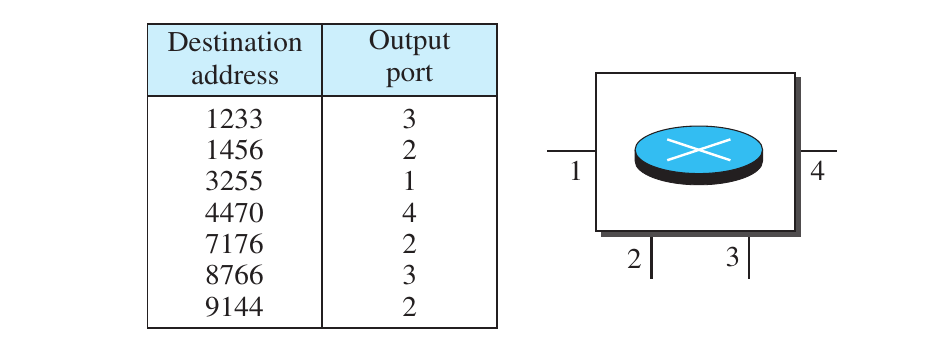
\includegraphics[scale=0.5]{8.27.png}
	\caption{8.27}
\end{figure}
\textbf{Find the output port for packets with the following destination addresses:}
\begin{enumerate}
	\item \textbf{ Packet 1: 7176 } Destination port: 2
	\item \textbf{ Packet 2: 1233 } Destination port: 3
	\item \textbf{ Packet 3: 8766 } Destination port: 3
	\item \textbf{ Packet 4: 9144 } Destination port: 2
\end{enumerate}

\subsection{Figure 8.28 shows a switch in a virtual-circuit network.}

\begin{figure}[H]
	\center
	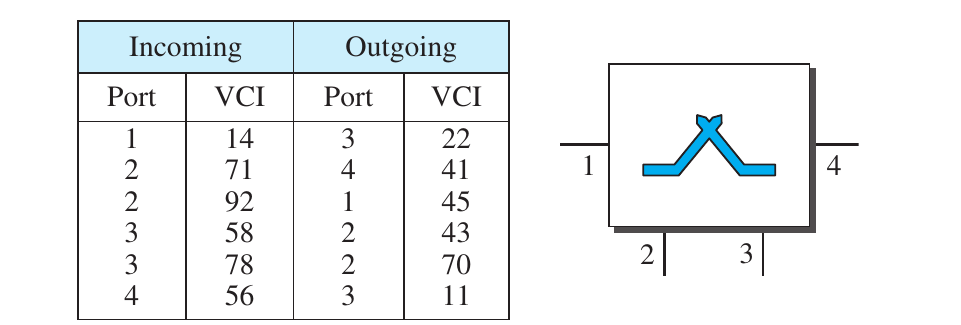
\includegraphics[scale=0.5]{8.28.png}
	\caption{8.27}
\end{figure}
\textbf{Find the output port for packets with the following destination addresses:}
\begin{enumerate}
	\item \textbf{ Packet 1: 3, 78 } Output port: 2, 70
	\item \textbf{ Packet 2: 2, 92 } Output port: 1, 45
	\item \textbf{ Packet 3: 4, 56 } Output port: 3, 11
	\item \textbf{ Packet 4: 2, 71 } Output port: 4, 41
\end{enumerate}

\subsection{Answer the following questions:}
\begin{enumerate}
	\item \textbf{ Can a routing table in a datagram network have two entries with the same
		      destination address? Explain.} \\
	      No, a routing table in a datagram network cannot have two entries with the same destination address. The routing table is used to find the output port from which the information belonging to a destination should be sent out. If there are two entries with the same destination address, the switch will not know which output port to use.

	\item \textbf{ Can a switching table in a virtual-circuit network have two entries with the
		      same input port number? With the same output port number? With the
		      same incoming VCIs? With the same outgoing VCIs? With the same incom-
		      ing values (port, VCI)? With the same outgoing values (port, VCI)?}
	      \begin{enumerate}
		      \item Yes, a switching table in a virtual-circuit network can have two entries with the same input port number. The input port number is used to identify the incoming port.
		      \item Yes, a switching table in a virtual-circuit network can have two entries with the same output port number. The output port number is used to identify the outgoing port.
		      \item Yes, a switching table in a virtual-circuit network can have two entries with the same incoming VCIs. The incoming VCIs are used to identify the incoming virtual circuit.
		      \item Yes, a switching table in a virtual-circuit network can have two entries with the same outgoing VCIs. The outgoing VCIs are used to identify the outgoing virtual circuit.
		      \item No, a switching table in a virtual-circuit network cannot have two entries with the same incoming values (port, VCI). The incoming values are used to identify the incoming port and virtual circuit.
		      \item No, a switching table in a virtual-circuit network cannot have two entries with the same outgoing values (port, VCI). The outgoing values are used to identify the outgoing port and virtual circuit.
	      \end{enumerate}
\end{enumerate}

\begin{theorem}
	In a virtual-circuit network, the VCIs are local. A VCI is unique only in rela-
	tionship to a port. In other words, the (port, VCI) combination is unique. This
	means that we can have two entries with the same input or output ports. We can
	have two entries with the same VCIs. However, we cannot have two entries
	with the same (port, VCI) pair.
\end{theorem}

\subsection{It is obvious that a router or a switch needs to search to find information in the
	corresponding table. The searching in a routing table for a datagram network
	is based on the destination address; the searching in a switching table in a
	virtual-circuit network is based on the combination of incoming port and
	incoming VCI. Explain the reason and define how these tables must be
	ordered (sorted) based on these values.}

In a datagram network, the searching in a routing table is based on the destination address. The routing table must be ordered (sorted) based on the destination address. \par In a virtual-circuit network, the searching in a switching table is based on the combination of incoming port and incoming VCI. The switching table must be ordered (sorted) based on the incoming port and incoming VCI. As port number is smaller, at first port number is used for sorting and then VCI is used for sorting.

\subsection{Consider an n × k crossbar switch with n inputs and k outputs.}

\textbf{
	\begin{enumerate}
		\item  Can we say that the switch acts as a multiplexer if n > k?
		\item Can we say that the switch acts as a demultiplexer if n < k?
	\end{enumerate}
} \par
Yes, we can say that the switch acts as a multiplexer if n > k. \par
Yes, we can say that the switch acts as a demultiplexer if n < k. \\
(But not always, details are discussed in any further chapter, I guess.)

\subsection{We need a three-stage space-division switch with N = 100. We use 10 cross-
	bars at the first and third stages and 4 crossbars at the middle stage.}

\begin{enumerate}
	\item \textbf{ Draw the configuration diagram. } \par
	      \begin{figure}[H]
		      \center
		      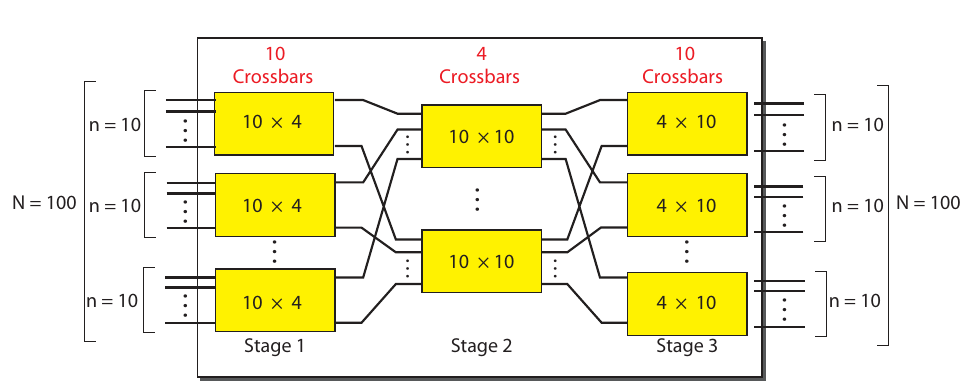
\includegraphics[scale=0.5]{8.1.png}
		      \caption{2.12}
	      \end{figure}
	\item \textbf{ Calculate the total number of crosspoints. } \\
	      Total number of crosspoints = $ 10 \times (10 \times 4) + 4 \times (10 \times 10) + 10 \times (10 \times 4) = 1200 $
	\item \textbf{ Find the possible number of simultaneous connections. } \\
	      As we have 10 crossbars at the first and third stages, and 4 crossbars at the middle stage,
	      more than 4 simultaneous connection is not possible for each first crossbar. \\
	      Possible number of simultaneous connections = $ 10 \times 4 = 40 $
	\item \textbf{ Find the possible number of simultaneous connections if we use a single crossbar (100 × 100). } \\
	      If we use a single crossbar, the possible number of simultaneous connections = $ 100 $.
	      Because we have 100 inputs and 100 outputs, so 100 simultaneous connections are possible.
	\item \textbf{ Find the blocking factor, the ratio of the number of connections in part c and in part d. } \\
	      Blocking factor = $ \frac{40}{100} = 0.4 $
\end{enumerate}

\subsection{Repeat Problem 8-12 if we use 6 crossbars at the middle stage.}

\begin{enumerate}
	\item \textbf{ Draw the configuration diagram. } \par
	      \begin{figure}[H]
		      \center
		      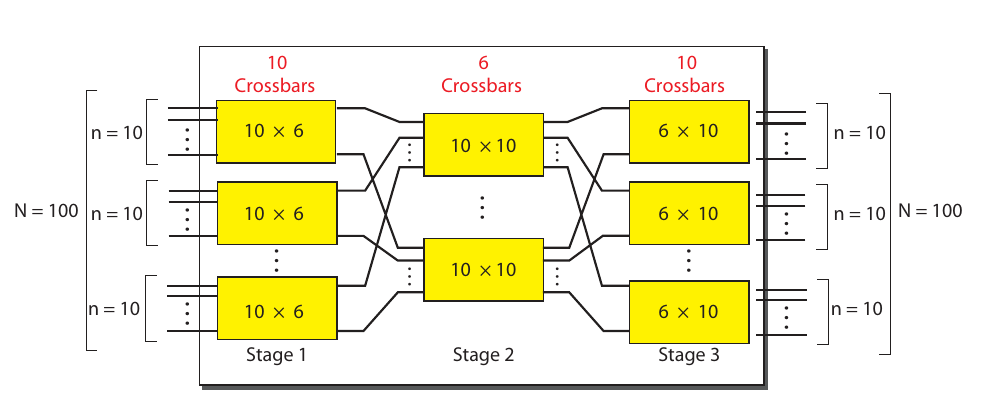
\includegraphics[scale=0.5]{8.2.png}
		      \caption{2.13}
	      \end{figure}
	\item \textbf{ Calculate the total number of crosspoints. } \\
	      Total number of crosspoints = $ 10 \times (10 \times 6) + 6 \times (10 \times 10) + 10 \times (10 \times 6) = 1800 $
	\item \textbf{ Find the possible number of simultaneous connections. } \\
	      As we have 10 crossbars at the first and third stages, and 6 crossbars at the middle stage,
	      more than 6 simultaneous connection is not possible for each first crossbar. \\
	      Possible number of simultaneous connections = $ 10 \times 6 = 60 $
	\item \textbf{ Find the possible number of simultaneous connections if we use a single crossbar (100 × 100). } \\
	      If we use a single crossbar, the possible number of simultaneous connections = $ 100 $.
	      Because we have 100 inputs and 100 outputs, so 100 simultaneous connections are possible.
	\item \textbf{ Find the blocking factor, the ratio of the number of connections in part c and in part d. } \\
	      Blocking factor = $ \frac{60}{100} = 0.6 $
\end{enumerate}

\subsection{Redesign the configuration of Problem 8-12 using the Clos criteria.}
According to clos, $ n = (N / 2)^{1/2} = 7.07 $. So we can choose n=8. \par
In this case, for the first and third stages, we need 8 crossbars,\\
and for the middle stage, we need k = 2n -1 = 15 crossbars. \par
Here's the configuration diagram:
\begin{figure}[H]
	\center
	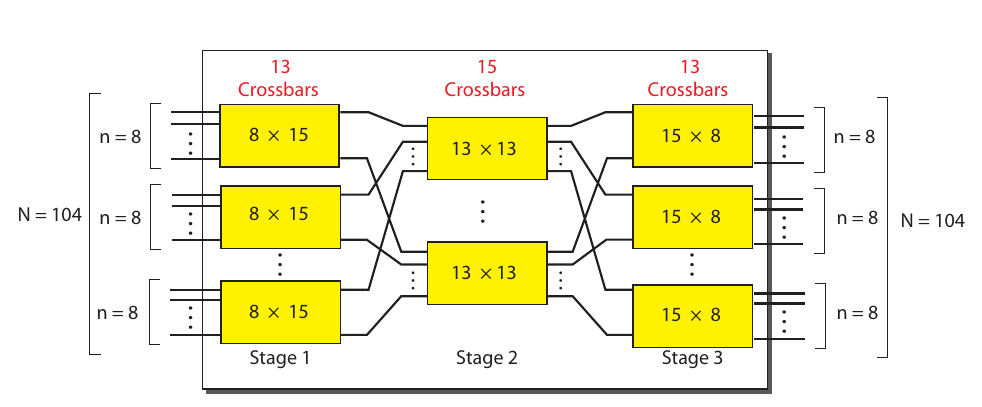
\includegraphics[scale=0.5]{8.3.png}
	\caption{2.14}
\end{figure}

So, our total number of crosspoints = $ 13 \times (8 \times 15) + 15 \times (13 \times 13) + 13 \times (15 \times 8) = 5655 $.
Which is less than with the case of 10,000 crosspoints $ (100 \times 100) $. As we can see, the clos criteria is more efficient.

\subsection{We need to have a space-division switch with 1000 inputs and outputs. What
	is the total number of crosspoints in each of the following cases?}
\begin{enumerate}
	\item \textbf{ Using a single crossbar. } \\
	      Total number of crosspoints = $ 1000 \times 1000 = 1000000 $
	\item \textbf{ Using a multi-stage switch based on the Clos criteria. } \\
	      According to clos, $ n = (N / 2)^{1/2} = 22.36 $. So we can choose n=23. \par
	      In this case, for the first and third stages, we need 23 crossbars,\\
	      and for the middle stage, we need k = 2n -1 = 45 crossbars. \par
	      So, our total number of crosspoints = $ 44 \times (23 \times 45) + 45 \times (23 \times 23) + 44 \times (45 \times 23) = 114885 $. (Not sure)
\end{enumerate}

\subsection{We need a three-stage time-space-time switch with N = 100. We use 10 TSIs
	at the first and third stages and 4 crossbars at the middle stage.}
\begin{enumerate}
	\item \textbf{ Draw the configuration diagram. }
	      \begin{figure}[H]
		      \center
		      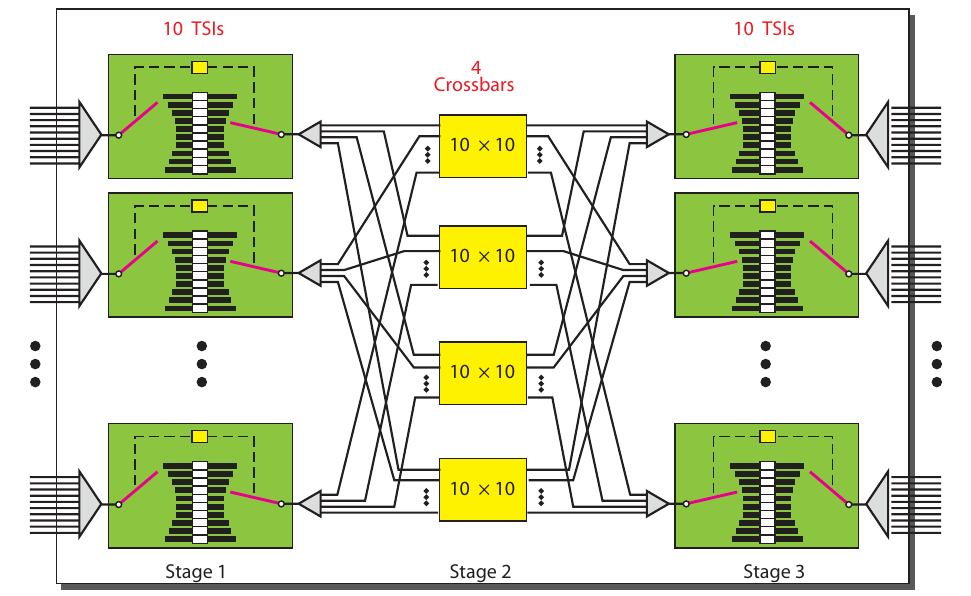
\includegraphics[scale=0.5]{8.4.png}
		      \caption{2.16}
	      \end{figure}
	\item \textbf{ Calculate the total number of crosspoints. } \\
	      Total number of crosspoints = $ 4 \times (10 \times 10) = 400 $
	\item \textbf{ Calculate the total number of memory locations we need for the TSIs. } \par
	      Total number of memory locations = $ 10 \times 10 + 10 \times 10 = 200 $
\end{enumerate}

\vspace{7.5cm}
\textbf{
	Anything can be a sword if you polish it enough.
}

\end{document}
